\documentclass[cjk,dvipdfmx,10pt,compress,fragile%
hyperref={bookmarks=true,bookmarksnumbered=true,bookmarksopen=false,%
colorlinks=false,%
pdftitle={第 134 回 関西 Debian 勉強会},%
pdfauthor={小林},%
%pdfinstitute={関西 Debian 勉強会},%
pdfsubject={資料},%
}]{beamer}

\title{自作キーボード温泉に日帰り入浴してみた話}
\author[Katsuki Kobayashi]{{\large\bf Katsuki Kobayashi}}
\institute[Debian JP]{{\normalsize\tt 関西 Debian 勉強会}}
\date{{\small 2019年 11月 24日 (日)}}

\usepackage{graphicx}
\usepackage{moreverb}
\usepackage{ulem}
\usepackage[varg]{txfonts}
\usepackage{tabularx}
\usepackage{fancybox}
\usepackage{fancyvrb}
\usepackage{float}
\usepackage{multicol}
\usepackage{minijs}
\usepackage{amsmath}
\usepackage{amssymb}
\usepackage{newtxtext}
\usepackage{listings}
\usepackage{xcolor}
\usepackage{hyperref}
\AtBeginDvi{\special{pdf:tounicode EUC-UCS2}}
\usetheme{KansaiDebian}
\def\museincludegraphics{%
  \begingroup
  \catcode`\|=0
  \catcode`\\=12
  \catcode`\#=12
  \includegraphics[width=0.9\textwidth]}
%\renewcommand{\familydefault}{\sfdefault}
%\renewcommand{\kanjifamilydefault}{\sfdefault}
%
\newenvironment{commandline}%
{\VerbatimEnvironment
  \begin{Sbox}\begin{minipage}{0.9\hsize}\begin{fontsize}{8}{8} \color{white} \begin{BVerbatim}}%
{\end{BVerbatim}\end{fontsize}\end{minipage}\end{Sbox}
  \setlength{\fboxsep}{8pt}
% start on a new paragraph

\vspace{6pt}% skip before
\fcolorbox{white}{black}{\TheSbox}

\vspace{3pt}% skip after
}
%end of commandline

\begin{document}

\begin{frame}[fragile]
\titlepage
\end{frame}

\begin{frame}[fragile,t]{お詫び}
 \begin{itemize}
  \item Debian要素はあんまりないです
 \end{itemize}
\end{frame}

\takahashi[40]{みなさん}
\takahashi[40]{肩や腰は\\大丈夫ですか?}
\takahashi[40]{私は駄目です}

\begin{frame}[fragile,t]{自作キーボードへの動機(1/4)}
 \begin{itemize}
  \item 会社にて腰痛が酷くて、対策しても効果がない
	\begin{itemize}
	 \item 整骨院に通う
	 \item ジムで筋トレする
	\end{itemize}
  \item 特に、ここ数年酷い
	\pause
  \item 心当たり
 \end{itemize}
\begin{center}
 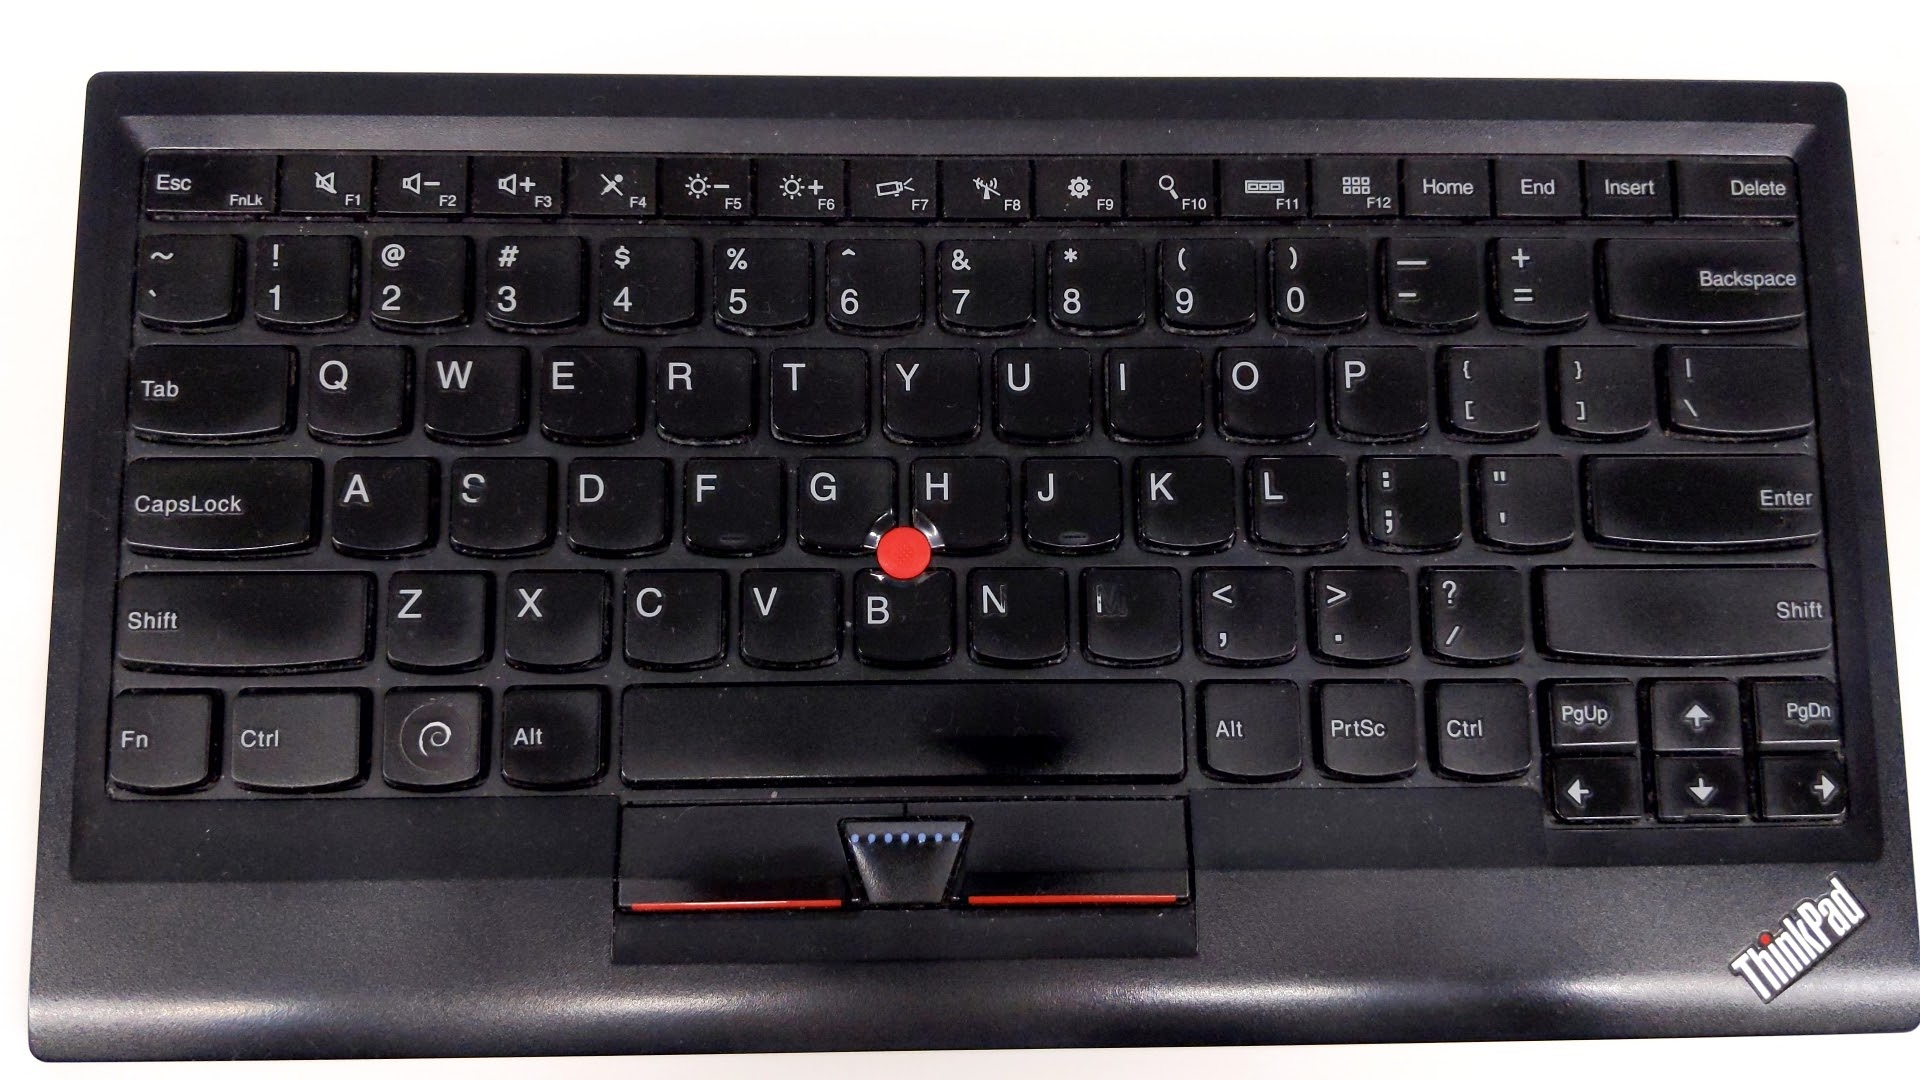
\includegraphics[keepaspectratio,height=4cm]{./img/thinkpad_kb.jpg}
\end{center}
\end{frame}

\begin{frame}[fragile,t]{自作キーボードへの動機(2/4)}
 \begin{itemize}
  \item ThinkPadキーボード
	\begin{itemize}
	 \item ThinkPadを使い始めて約4年
	 \item トラックポイントの良さに気付いて会社でもThinkPadキーボードに
	       \begin{itemize}
		\item WindowsではLinuxほど恩恵には預かれないけど
	       \end{itemize}
	 \item トラックポイントが悪いのかと思い、ここ数ヶ月はマウスを使用
	       \begin{itemize}
		\item しかし改善せず……
	       \end{itemize}
	\end{itemize}
	\pause
  \item 分割型キーボード
	\begin{itemize}
	 \item まぁ、肩凝りには効きそう
	 \item しかし、腰に効くのか想像できない
	\end{itemize}
 \end{itemize}
\end{frame}

\begin{frame}[fragile,t]{自作キーボードへの動機(3/4)}
 \begin{itemize}
  \item \href{https://ultimatehackingkeyboard.com/}{Ultimate Hacking Keyboard}なるものをみつける
	\begin{itemize}
	 \item トラックポイントが付く!!
	       \begin{itemize}
		\item しかし場所がおかしい
		\item トラックボールやタッチパッドも付けられる
	       \end{itemize}
	 \item 軸は変更できる
	       \begin{itemize}
		\item 軸については後ほど……
	       \end{itemize}
	 \item ファームもカスタマイズできる
	 \item でもお値段的に
	       \begin{itemize}
		\item 最小構成でも275ドル
		\item トラックポイントつけたらいレストアームつけると4万円越え
	       \end{itemize}
	\end{itemize}
 \end{itemize}
\end{frame}

\begin{frame}[fragile,t]{自作キーボードへの動機(4/4)}
 \begin{itemize}
  \item 沼の住人からお声かけいただく
	\begin{itemize}
	 \item \url{https://twitter.com/rarewin/status/1163656414184689665}
	\end{itemize}
  \item \href{https://mechanicalkeyboards.com/shop/index.php?l=product_detail&p=3532}{Tex Yoda II}
	\begin{itemize}
	 \item 分割されてたら求めていた感じだった
	\end{itemize}
  \item 自作キーボードにトラックポイントを付けている人は一定数いるらしい
	\begin{itemize}
	 \item \href{https://www.google.com/search?client=firefox-b-e&q=%E3%83%88%E3%83%A9%E3%83%83%E3%82%AF%E3%83%9D%E3%82%A4%E3%83%B3%E3%83%88+%E8%87%AA%E4%BD%9C%E3%82%AD%E3%83%BC%E3%83%9C%E3%83%BC%E3%83%89}{Google検索: トラックポイント 自作キーボード}
	\end{itemize}
  \item そんなこんなで、自作へと心が……
 \end{itemize}
\end{frame}

\begin{frame}[fragile,t]{キーボードの選定(1/)}
 \begin{itemize}
  \item この業界では、自分の追い求めた理想のキーボードを \textbf{Endgame} というそうです
  \item 個人的に試したかったもの
	\begin{itemize}
	 \item 分割キーボード - 肩凝りに効きそうだったので必須
	 \item なるべく普通な配列 - 格子配列とかはひとまず避けたい
	 \item 打鍵音は静かなのがいい
	 \item トラックポイント欲しい……が、一旦あきらめる
	\end{itemize}
 \end{itemize}
\end{frame}

\begin{frame}[fragile,t]{キーボードの選定(2/)}
 \begin{itemize}
  \item 考えるべき事はいくつかある
  \item 各キーの配列はファームウェアがあるのでなんとでもなる
	\begin{itemize}
	 \item QWERTY配列とDvorak配列を切り替えられるようなファームもある
	\end{itemize}
  \item キーの配置
	\begin{itemize}
	 \item 普通の
	 \item 格子状 -- 省スペース! (代表: \href{https://yushakobo.jp/shop/helix-keyboard-kit/}{Helix})
	 \item エルゴノミクス -- 指の長さや親指の稼動域を考慮 (代表: \href{ErgoDox}{https://ergodox-ez.com/})
	\end{itemize}
  \item キーの数
	\begin{itemize}
	 \item XX\%キーボード -- フルキー(104キー)に対して何個のキーがあるか
	       \begin{itemize}
		\item 主流は60\%くらい (数字キーの段あり、テンキー、FunctionKeyなし)
		\item さらにいくと40\%くらい (数字キーなし、カーソルキーや一部記号キーなし)
		\item \href{https://www.reddit.com/r/MechanicalKeyboards/comments/dnrvz8/science_isnt_about_why_its_about_why_not/}{あたまおかしいの 10\%}
		\item 逆に100を越えるのも(ゲーム用とか)
	       \end{itemize}
	\end{itemize}
 \end{itemize}
\end{frame}

\begin{frame}[fragile,t]{キースイッチ(1/)}
 \begin{itemize}
  \item 現状、普及しているのは以下の2種類?
	\begin{itemize}
	 \item Cherry MX (左)  - ドイツCherry社
	       \begin{itemize}
		\item 特許が切れているためクローンがいっぱいある模様 (Gateron等)
		\item 出回っているキットはほとんど対応
		\item 最近ロープロファイルが出た? \href{https://www.cherrymx.de/en/mx-low-profile/mx-low-profile-red.html}{参考}
	       \end{itemize}
	 \item Kailh ロープロファイル (右) - 中国のKaihua?
	       \begin{itemize}
		\item Cherry MXとは互換性がない(対応している基板が必要)ので注意が必要
	       \end{itemize}
	\end{itemize}
  \item みなさんご存知の通り、色によって押し具合が変わる
 \end{itemize}
 \begin{center}
  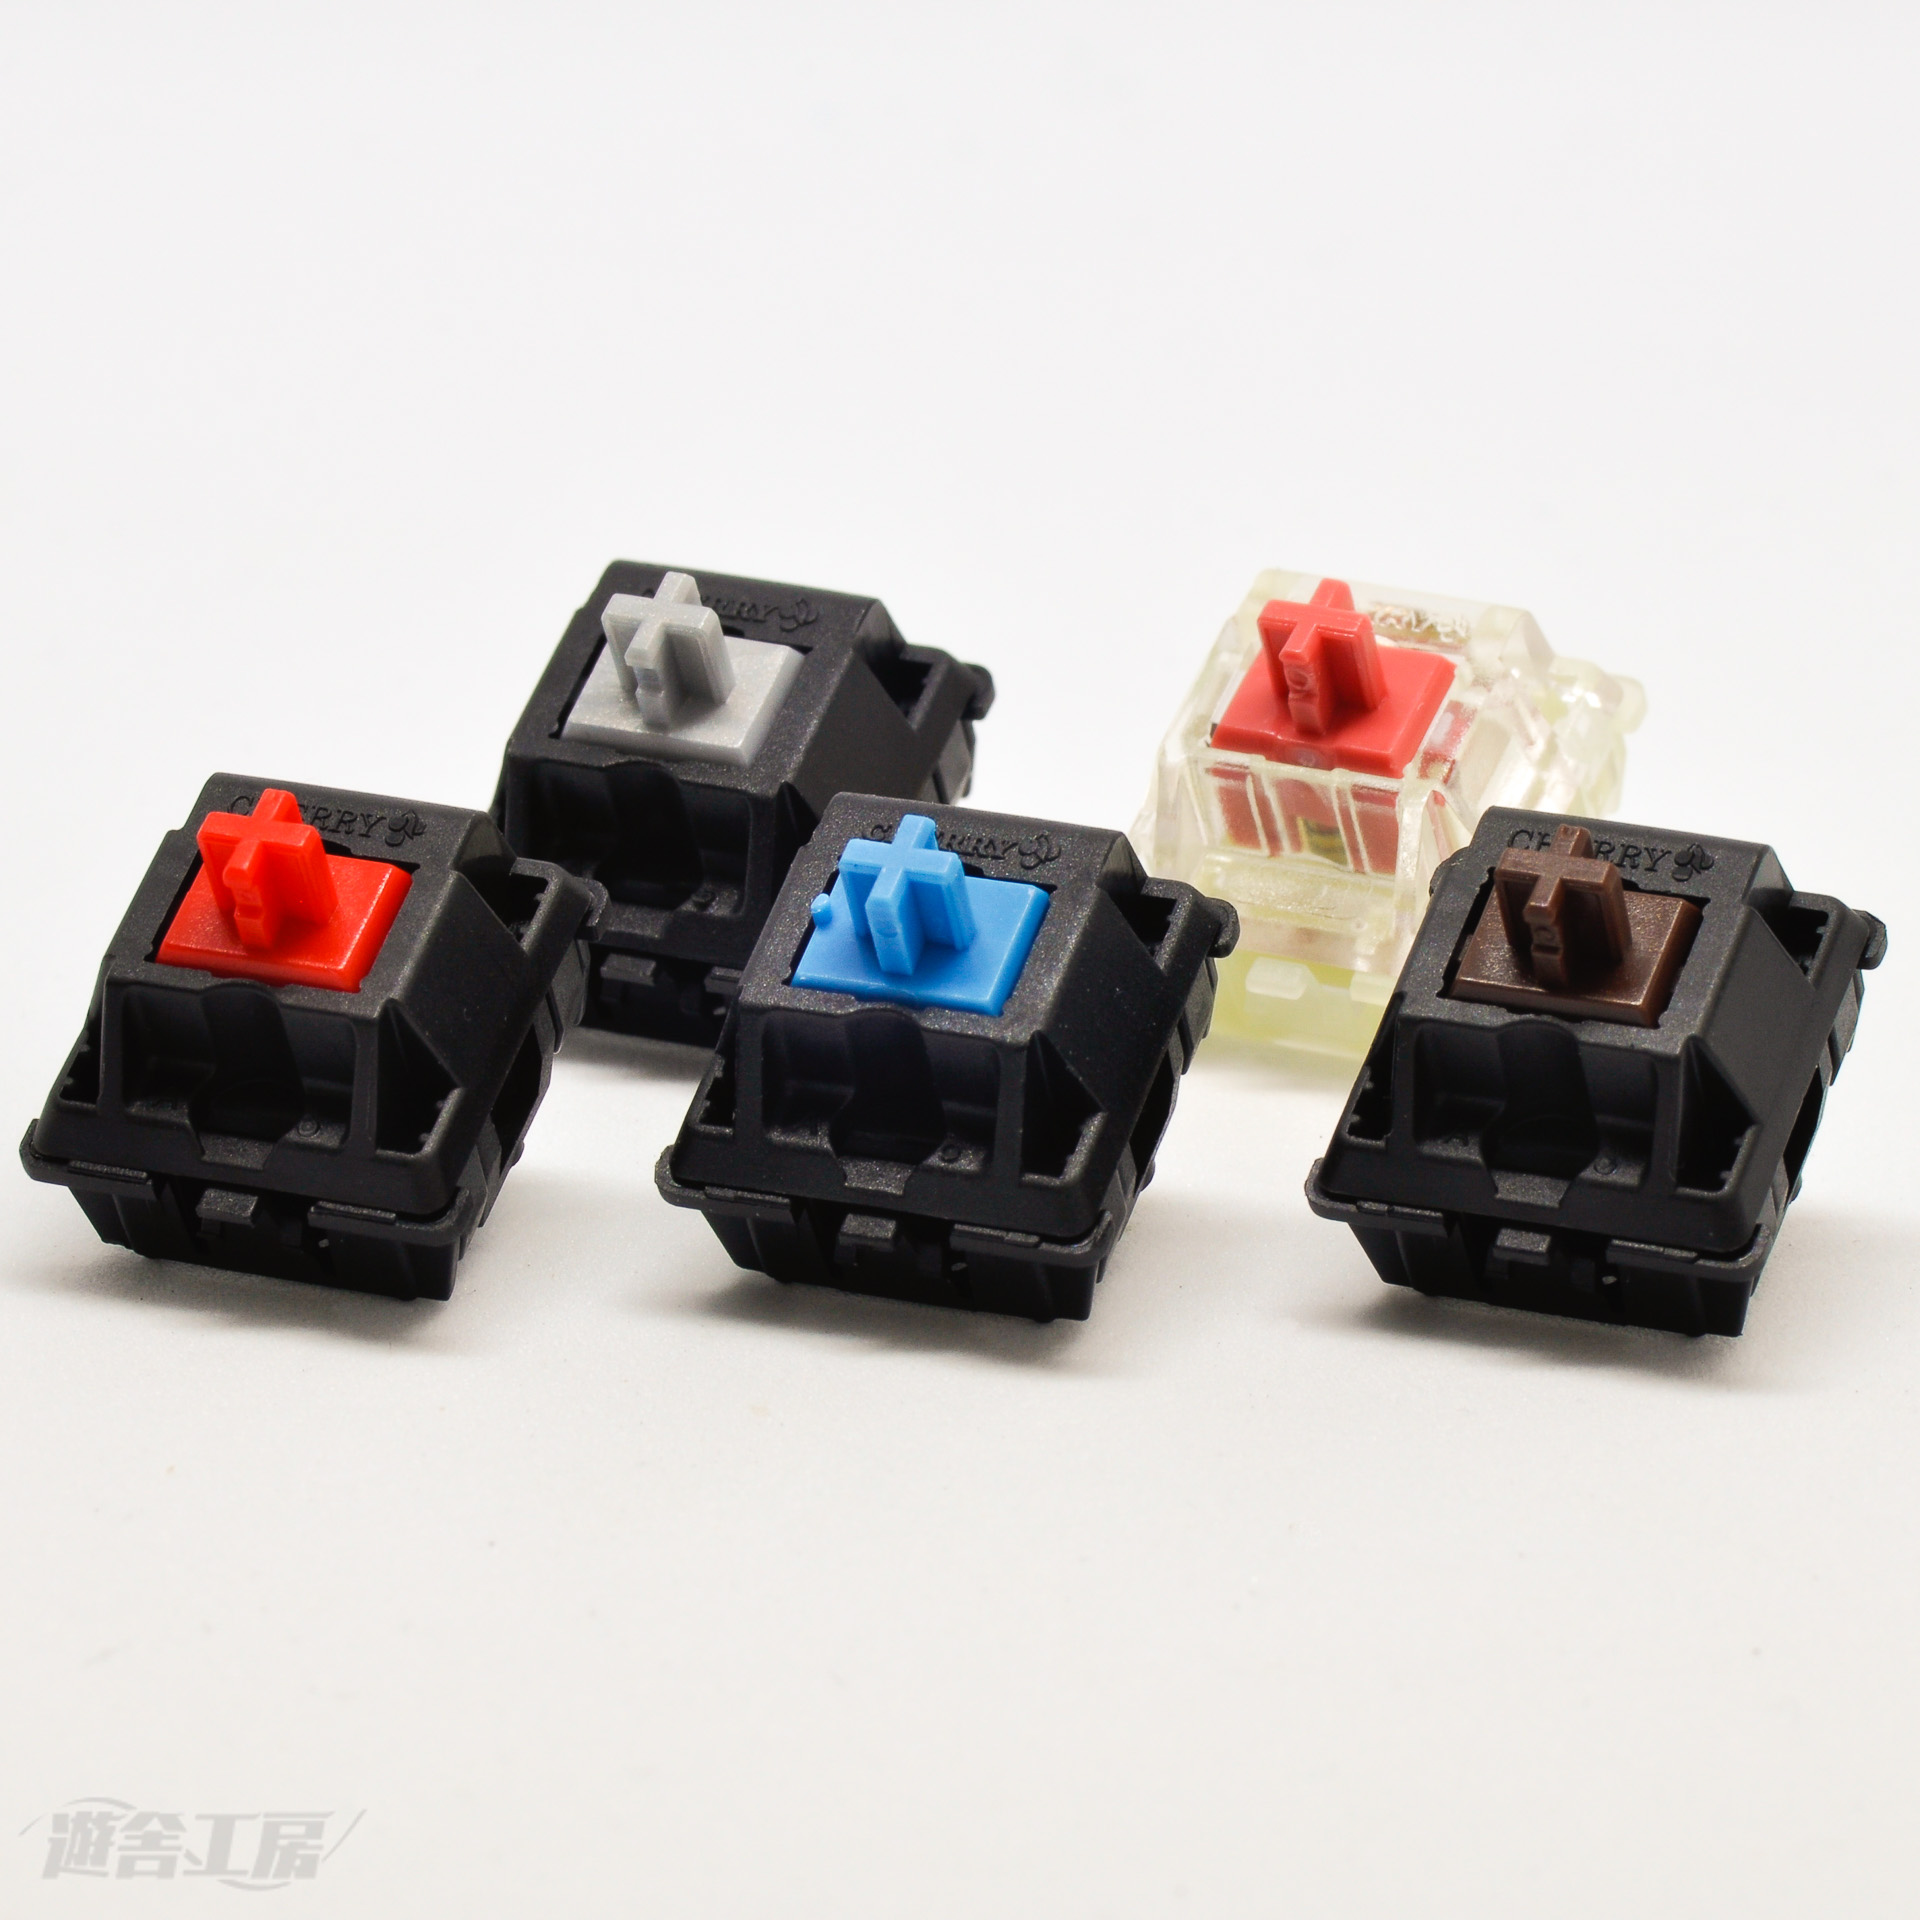
\includegraphics[keepaspectratio,height=3cm]{./img/Cherry_MX-1.jpg}
  \hspace*{1zw}
  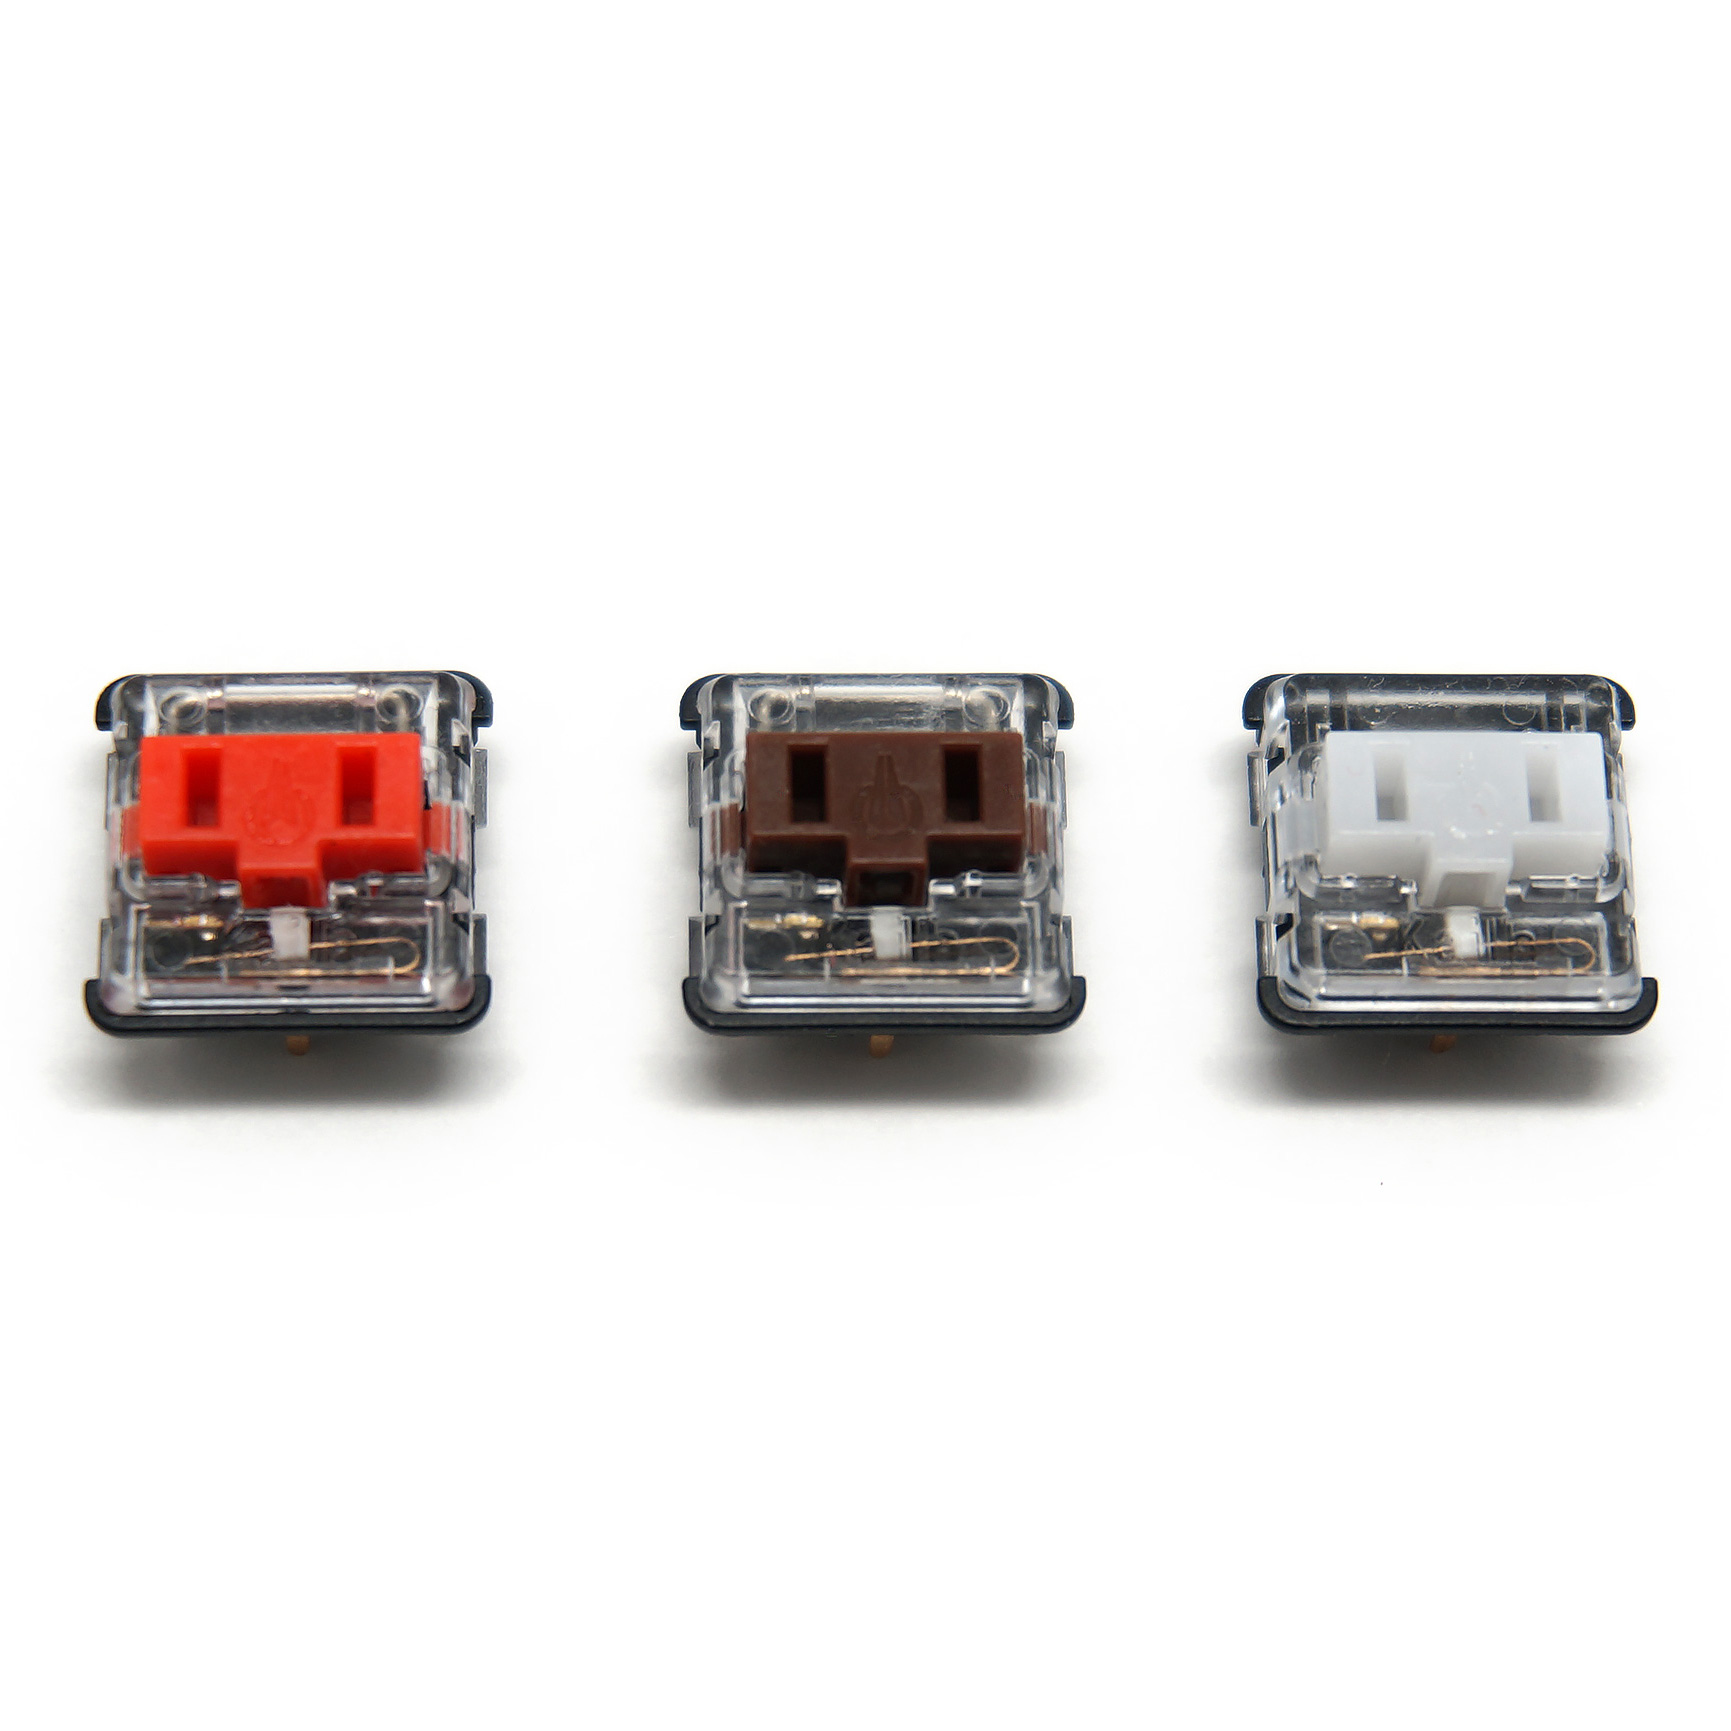
\includegraphics[keepaspectratio,height=3cm]{./img/YKB0003S.jpg}
 \end{center}
 \vspace{-1zw}
 \begin{flushright}
  \footnotesize
  引用元: \url{https://yushakobo.jp/shop/cherry-mx/}, \url{https://yushakobo.jp/shop/pg1350/}
 \end{flushright}
\end{frame}

\begin{frame}[fragile,t]{キースイッチ(2/)}
 \begin{center}
  \begin{tabular}[tb]{c|cccc}
   軸       & クリック感 & 音       & 重さ   & 深さ \\ \hline
   ピンク軸 & なし       & しずか   & かるめ\\
   赤軸     & なし       & ふつう   & かるめ\\
   茶軸     & あり       & ふつう   & ふつう\\
   黒軸     & なし       & ふつう   & おもめ \\
   青軸     & あり       & カチカチ & おもめ \\
   銀軸     &            &          &        & 浅め
  \end{tabular}
 \end{center}
 \begin{flushright}
  参考: \url{https://www.diatec.co.jp/products/CHERRY/}
 \end{flushright}
\begin{itemize}
 \item 既製品だと全体同じ軸だが、 \textbf{自作だと自由自在}
       \begin{itemize}
	\item 小指周りは軽めのスイッチを配置したり
	\item \href{https://yushakobo.jp/shop/a01ps/}{ソケット}を付けておいて後で変更できるようにしたり
       \end{itemize}
\end{itemize}
\end{frame}

\begin{frame}[fragile,t]{マイコン}
 \begin{itemize}
  \item \href{https://www.sparkfun.com/products/12640}{Sparkfun社が出している} Arduino互換ボード
	\begin{itemize}
	 \item とてもコンパクトだけどピン数は結構ある
	 \item ArduinoのIDEが使える
	 \item 定価は結構おたかめ…… \$19.95
	\end{itemize}
  \item Promicroの互換品を使うのが現在の主流
	\begin{itemize}
	 \item おやすい (クローン品だと500円とかで手に入る)
	 \item 情報が多いく、キーボードFW用のフレームワークがある(後述)
	\end{itemize}
 \end{itemize}
\end{frame}

\begin{frame}[fragile,t]{一般的な自作キーボードの構成}
\end{frame}

\begin{frame}[fragile,t]{Mint60}
 \begin{itemize}
  \item 一台目として購入 (\href{https://eucalyn.shop/shop/kits/mint60-starter}{公式販売サイト})
	\begin{itemize}
	 \item オーソドックスな分割60\%キーボード
	 \item キースイッチ/キャップ付きのキットがあって購入しやすい
	       \begin{itemize}
		\item 大体のキットは、スイッチとキーキャップは別途用意する
	       \end{itemize}
	 \item 組み立ての難易度も低い
	       \begin{itemize}
		\item 半田付け難易度の高い素子(チップダイオード/チップLEDなど)はない \pause
		\item ただし、発表者は未だにシリアル通信が動いていない
	       \end{itemize}
	\end{itemize}
 \end{itemize}
\end{frame}

\takahashi[30]{それでも満足できない\\アナタへ}
\takahashi[30]{プリント基板自作手順}

\begin{frame}[fragile,t]{PCB(1/)}
 \begin{itemize}
  \item 茶番は終わって本題に入ります \pause
  \item ここまで見てきてわかったと思いますが \pause
  \item 完璧なキットがみつからなければエンドゲームはあり得ません
 \end{itemize}
\end{frame}

\begin{frame}[fragile,t]{キースキャン回路}
\end{frame}


\end{document}